 Um esquema útil para organização é a classificação de Layman. Denomina-se

\begin{enumerate}
	\item \textbf{Entradas Independentes}: Adicionada a necessidade de simetria, matrizes deste tipo são chamadas matrizes de Wigner.
	\item \textbf{Invariantes por rotação}: Quaisquer duas matrizes que são relacionadas por uma transformação $\matriz{H'} = \matriz{U} \matriz{H} \matriz{U}^{-1}$ ocorrerão com a mesma probabilidade.
\end{enumerate}

Só existe um tipo especial de matriz que se encontra na intersecção e são as classes Gaussianas.

Em geral no mundo das matrizes aleatórias três classes são muito importantes e serão atores centrais no nosso estudo. São as três classes associadas às matrizes que tem entradas gaussianas. Estas são: O Ensemble Gaussiano Ortogonal (GOE), O Ensemble Gaussiano Unitário (GUE) e o Ensemble Gaussiano Simplético (GSE). Em suma, eles tratam, em ordem, de matrizes com entradas gaussianas reais, complexas e quaterniônicas. Seus nomes estão relacionados com a matriz necessária para a transformação de diagonalização das matrizes. Unitária para o caso complexo, por exemplo. Seus autovalores possuem distribuições distintas (ao menos para a escala usada) e é ilustrada abaixo na Figura \ref{fig: lambdadist}.

\begin{center}
	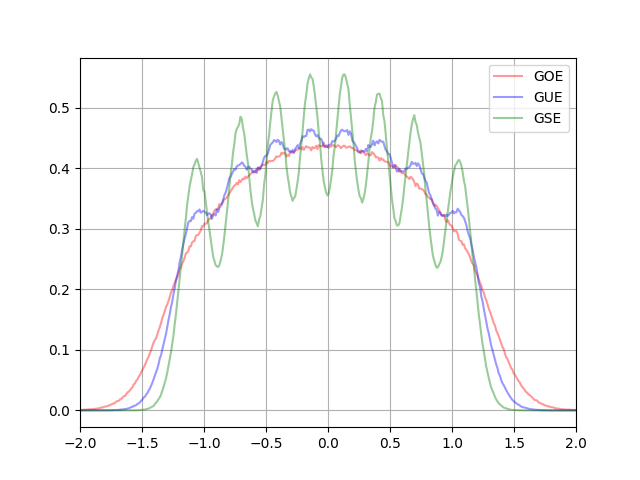
\includegraphics[width=0.8\linewidth]{FullGaussianDensityEscaled.png}
	\label{fig: lambdadist}
\end{center}

Mais desenvolvimento sobre a forma desta distribuição e as diferenças será feito posteriormente. Usaremos a referência \cite{Livan_2018} para a maior parte dos desenvolvimentos. Algum material interessante pode ser consultado em um livro de física em \cite{MEHTA1967v}.